\documentclass{beamer}
\usetheme{Darmstadt}
\usecolortheme{beaver}
\usepackage{booktabs}
\usepackage{hyperref}

\usepackage[utf8]{inputenc}
\usepackage{graphicx}
\graphicspath{ {./images/} }

%Information to be included in the title page:
\title{Sample title}
\author{Brandon Hosley}
\institute{University of Illinois - Springfield}
\date{\today}

\begin{document}
\frame{\titlepage}

\begin{frame}{Overview}
\tableofcontents
\end{frame}

\section[Q1]{Q1: Bias–variance tradeoff}

\begin{frame}{Bias-Variance Trade-Off}
	\begin{columns}
		\column{0.5\textwidth}
		Bias Error
		\begin{itemize}
			\item<1-> Also called 'Overfitting'
			\item<4-> Predicts test data too well
		\end{itemize}
		
		\column{0.5\textwidth}
		Variance 
		\begin{itemize}
			\item<2-> Also called 'Underfitting'
			\item<5-> Generalizes too well
		\end{itemize}
	\end{columns}
	\centering
	\onslide<3->{\includegraphics[width=0.6\linewidth]{OverAndUnderFit}}
\end{frame}

\begin{frame}{Bias-Variance Trade-Off}
	Aiming for the lowest possible error typically means finding a "middle-ground" \\
	A common technique for this is determining the minimum \emph{mean squared error.} \\
	\begin{align}
		\text{MSE} &= \left( E\left[\hat{f}(x)\right]-f(x)\right) + E\left[\left(\hat{f}(x) - E\left[\hat{f}(x)\right]\right)^2\right] +
		\sigma^2_e \\
		&= \text{Bias}
	\end{align}
	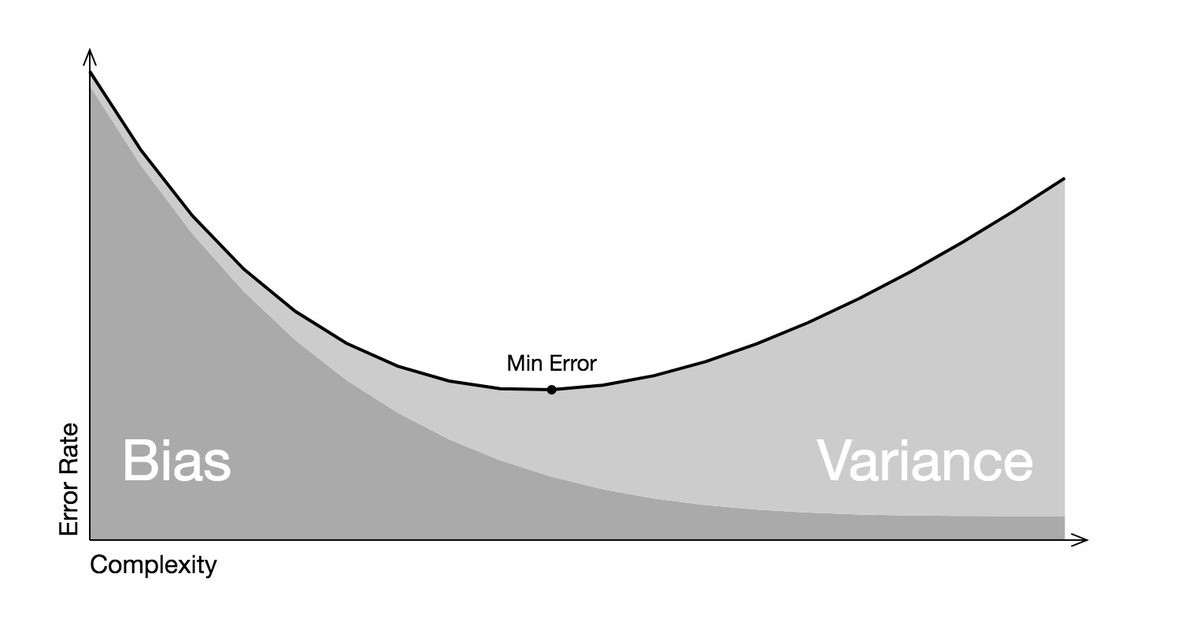
\includegraphics[width=0.5\linewidth]{MinError}
\end{frame}

\section[Q2]{Q2: Hastie and Tibshirani}
\section[Q3]{Q3: ISL Section 2.3}
\section[Q4]{Q4: ISL Section 2.4}
%Exercises. No. 10 (p. 56)

\end{document}
